\documentclass[12pt]{article}

\usepackage[a4paper, margin=1in]{geometry}
\usepackage{xcolor}
\usepackage{tcolorbox}
\usepackage{fontawesome5} % icons
\usepackage{hyperref}
\usepackage{graphicx}
\usepackage{float}
\usepackage{comment}
\usepackage[nameinlink,capitalize,noabbrev]{cleveref}
\usepackage{subcaption} % modern replacement for the deprecated subfigure package

\setlength{\parindent}{0pt}

% --- COLOR PALETTE (customize these) ---
\definecolor{maincolor}{HTML}{2A9D8F} % your teal
\definecolor{accentcolor}{HTML}{E76F51}
\definecolor{lightcolor}{HTML}{FFDEAD}

% Tell cleveref how to name your counter
\crefname{exercise}{assignment}{assignments}
\Crefname{exercise}{Assignment}{Assignments}

% --- ASSIGNMENT STYLE ---
\newcounter{exercise}

% Optional label: \exercisetitle[<label>]{<Title>}
\newcommand{\exercisetitle}[2][]{%
  \refstepcounter{exercise}% make this step referenceable/hyperlinked
  \vspace{0.5cm}%
  \colorbox{maincolor}{%
    \makebox[\dimexpr\linewidth-2\fboxsep][l]{%
      \textcolor{white}{\faPen\ Assignment \theexercise:~ #2}%
    }%
  }%
  % If an optional label was provided, set it
  \if\relax\detokenize{#1}\relax\else\label{#1}\fi
  \vspace{0.3cm}%
}


% --- IMPORTANT BOX ---
\newtcolorbox{importantbox}{
  colback=lightcolor,
  colframe=accentcolor,
  arc=4mm,
  boxrule=1pt,
  left=6pt,
  right=6pt,
  top=6pt,
  bottom=6pt
}

% --- PROMPT BOX ---
\newtcolorbox{promptbox}{
  colback=white,
  colframe=maincolor,
  arc=4mm,
  boxrule=1pt,
  left=6pt,
  right=6pt,
  top=6pt,
  bottom=6pt
}

% --- QUESTION BOX (with starred variant and cleveref names) ---
% Requires: \usepackage{hyperref} for \Form/\TextField
%           \usepackage{fontawesome5} for \faEdit

% Cleveref names for the question counter
\crefname{question}{question}{questions}
\Crefname{question}{Question}{Questions}

\makeatletter
\newcounter{question}
\newlength\questionheight
\setlength\questionheight{5cm} % default answer box height

% \question{<text>}                  -> with TextField (default height)
% \question[<height>]{<text>}        -> with TextField (custom height)
% \question*{<text>}                 -> no TextField, still numbered
\newcommand{\question}{\@ifstar{\question@text}{\question@field}}

% Common heading (increments counter and creates ref anchor)
\newcommand{\question@heading}[1]{%
  \refstepcounter{question}%
  \vspace{0.3cm}%
  \noindent\textbf{\faEdit\ Question \thequestion: #1}%\\[0.3em]%
}

% Starred form: numbered question without input field
\newcommand{\question@text}[1]{%
  \question@heading{#1}%
%  \vspace{0.3cm}%
}

% Unstarred form: numbered question with input field (optional height)
\newcommand{\question@field}[2][\questionheight]{%
  \question@heading{#2}%
 \\[0.3em] \begin{Form}
    \TextField[
      name=Q\thequestion,
      multiline=true,
      width=\linewidth,
      height=#1,
      charsize=10pt,
      bordercolor={0 0 0},
      borderwidth=1.8,
      backgroundcolor={1 1 1}
    ]{}
  \end{Form}
  \vspace{0.3cm}%
}
\makeatother

% --- SOLUTION BOX ---
%--- Definition of solution/no solution env to change between the teacher and the student versions --------%

% --- Teacher toggle ---
\newif\ifteacher
\teacherfalse  % Write teacherfalse for student version and teachertrue for teachers version

% --- Solution environment ---
\newtcolorbox{solutionbox}{colback=gray!10,colframe=black!60!black,arc=1mm,boxrule=1pt}

\ifteacher
\newenvironment{solution}{%
  \begin{solutionbox}\textbf{Solution:}
}{%
  \end{solutionbox}
}
\else
  \excludecomment{solution}
\fi


\begin{document}

\begin{titlepage}

% --- Top spacing ---
\vspace*{2cm}

% --- Title page ---
\begin{center}
    {\Huge \bfseries \color{maincolor} How does a large language model (LLM) work? \par}
    \vspace{0.5cm}
    
    {\Large \color{accentcolor} Teaching with AI (TAI) \par}
    
    \vspace{1.5cm}
    
    \begin{center}
{\large
Mirte van der Eyden$^{1}$, Andrea López Incera$^{2}$ \\[0.3cm]

{\small
$^{1}$ Institut für Fachdidaktik, Universität Innsbruck \\ 
mirte.van-der-eyden@uibk.ac.at \\[0.2cm]


$^{2}$ Departament de didàctica de la matemàtica i les ciències experimentals, Universitat Autònoma de Barcelona \\ 
andrea.lopez.incera@uab.cat
}
}
\end{center}

\end{center}

\vfill

% --- Logos at the bottom ---
\begin{center}
\begin{tabular}{ccc}

\includegraphics[height=1.5cm]{Figures/Logos/universitaet-innsbruck-logo-cmyk-farbe.jpg} &

\includegraphics[height=1.5cm]{Figures/Logos/logotipuab-v1-verd.png} &

\includegraphics[height=1.5cm]{Figures/Logos/EN Co-funded by the EU_POS.jpg}
\end{tabular}
\end{center}


\vspace{0.5cm}

% Optional footer text
\begin{center}
    {\small Project funded by Erasmus+ Programme of the European Union}
\end{center}

\end{titlepage}

% --- Description of activity ---
\vspace*{0.5\textheight}

Subject: Any subject for which you use an LLM, or specific subjects like technology.

\vspace{0.3cm}
\textbf{No background on science or technology needed!}

Note: we recommend that before doing this activity, the students do an unplugged activity in which they get familiar with the idea of predicting a word to complete a sentence. We recommend doing an ``exquisite corpse'' (folded story) game, in which a student has to complete a sentence that another student started writing, having access only to the last words of the sentence. At the end, a paragraph, or short text is created. 
\vspace{0.3cm}

Activity duration: 45 min

\vspace{0.5cm}

Steps:
\begin{enumerate}
    \item Word embeddings (10 min)
    \item Introducing context (10 min) 
    \item Be an LLM (25 min)
\end{enumerate}

Learning goals:

\begin{itemize}
    \item Understand the basics behind LLMs: how they work and how they are trained.
    \item Secondary goal: one first needs to understand how they work to then understand why they fail in certain things, which answers to trust and which not to trust, etc.

\end{itemize}

\newpage

% --- HEADER / BRANDING ---
\begin{center}
    {\LARGE \color{maincolor} How does a large language model (LLM) work?}\\[5pt]
    {\large \textit{Learn the inner workings of ChatGPT, Claude, Gemini, etc.}}\\
    \rule{\linewidth}{1pt}
\end{center}

\vspace{0.5cm}

\textit{Have you ever wondered how a machine generates answers for your questions? How does it ``think"?
}
\vspace{0.3cm}

You will go through the same steps and mechanisms that an LLM uses to generate text. Like an LLM, your goal will be to generate the word that follows in an incomplete sentence.

% --- Assignment ---
\exercisetitle{Word embeddings}

Machines cannot recognize words like us. Instead, they need representations of those words with numbers. More specifically, each sentence is split into tokens and each token is then transformed or ``embedded" into a vector in a vector space of a very big dimension, one that you cannot draw anymore in 2D or 3D. In the exercises below, we will make a simplification and do some exercises in 2D to be able to visualize the ideas.

\question*{Have a look at the following link \hyperlink{maincolor}{https://tiktokenizer.vercel.app/} to see how an LLM splits sentences into tokens.}

\vspace{0.3cm}
\textcolor{maincolor}{\textbf{\faPen\ Instructions for Question 1.}} Write a sentence on the field on the right of ``System" and you will see the sentence splitting that the machine creates on the right. Each part is marked with a color and is assigned a token number that you can see in the box below. If you hover with your mouse over a text piece, you will see the number that corresponds to it in the box below, marked with the same color. Those numbers identify the tokens. Then, each token will have a vector embedding. But we will learn about those in the exercises below.

\begin{importantbox}
    Machines cannot recognize words like us. Instead, they need representations of those words with numbers.
\end{importantbox}

Note: in the exercises below, we will ignore the transformation into tokens, since for us humans, it is easier to work with words directly.

\vspace{0.5cm}

\textcolor{maincolor}{\textbf{\faPen\ a) Place the following words (use pencil!) on the grid below, grouping them by meaning.}} If you think two or more words are related in some way, place them close together. Otherwise, place them far away from each other. The word cat is already placed as an example. Don't forget to mark the bullet point for each of the words. 

\vspace{0.3cm}
\textbf{Words:} \textit{cat, wolf, horse, dog, zebra, tiger}


\begin{figure}[H]
    \centering
			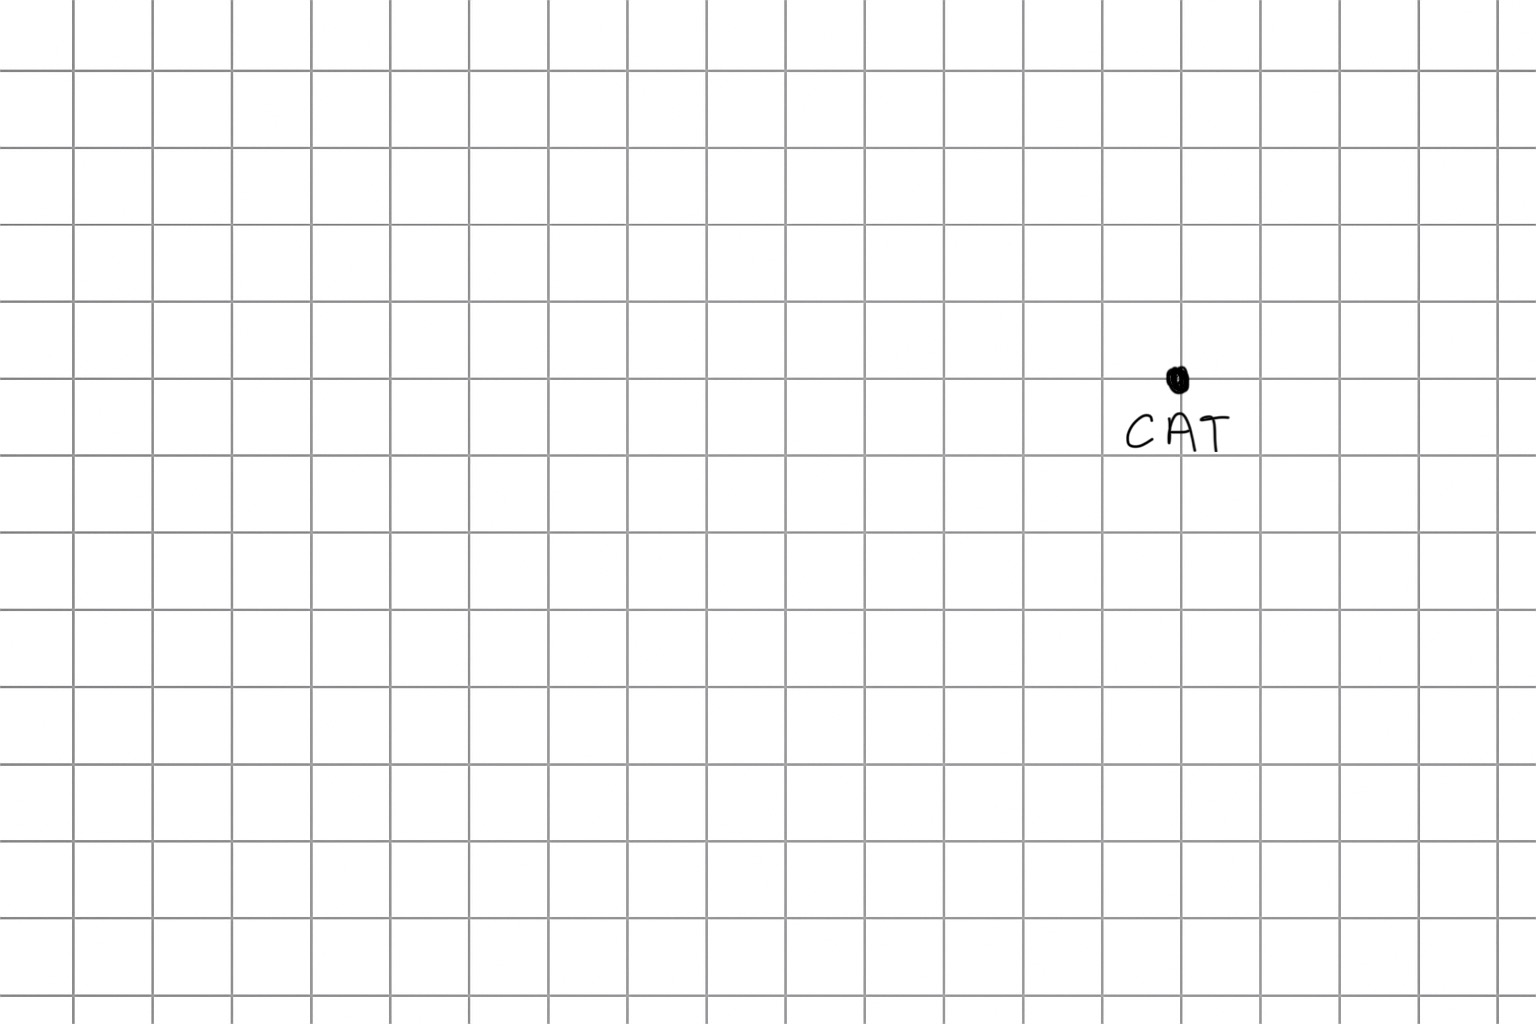
\includegraphics[width=\textwidth]{Figures/LLMs_work/grid_gpt_generated_example.jpg}
\end{figure}

\begin{solution}
    There is not a unique solution. The idea here is that the student groups the words together into clusters depending on the meaning. One possibility is that domestic animals are grouped together in one cluster (cat, horse, dog) and wild animals are grouped together in a separate cluster (tiger, zebra, wolf).
\end{solution}


In the following picture, we added the words \textbf{kitten, puppy and foal}, which are the baby versions of cat, dog and horse respectively. This relation is indicated by the arrows. Note that all arrows have the same direction (inclination).

\begin{figure}[H]
    \centering
			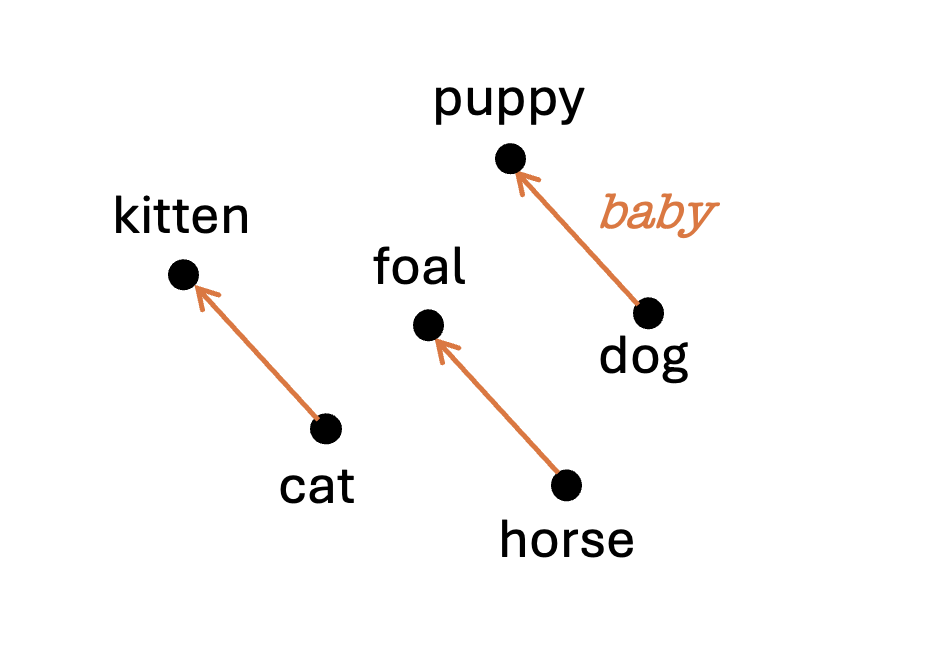
\includegraphics[width=\textwidth]{Figures/LLMs_work/example_babyvector_animals.png}
\end{figure}

\textcolor{maincolor}{\textbf{\faPen\ b) Can you find an analogous relation between the groups of words you placed in the grid above?}} If you do, connect with an arrow the pairs of words that follow this relation in the grid above. Note that you may need to move the words you already placed to make sure that all the arrows indicating the relation have the same direction (inclination).

\question{In the picture, the relation has the meaning of ``baby". What is the meaning of the relation between your groups of words (also called clusters)?}

\begin{solution}
    the analogous relation to ``baby" is ``wild version":

The wild version of the cat is the tiger

The wild version of the dog is the wolf

The wild version of the horse is the zebra

Therefore, cat and tiger need to be connected by an arrow (from cat to tiger), and analogously for dog - wolf and horse - zebra.
\end{solution}

\begin{importantbox}
    After splitting the sentence into tokens, the LLM learns to transform or ``embed" each token into a grid, grouping them by meaning, as you did above. However, the LLM's grid is of much higher dimension than 2D or 3D, and cannot be drawn anymore. In this grid, meaning relations (like ``baby version'' or ``wild version") are arrows.
\end{importantbox}

\vspace{0.5cm}

% --- Assignment  ---
\exercisetitle{ Introducing context}

\textcolor{maincolor}{\textbf{\faPen\ a) Given the clusters of words below, place the word \textit{mole} in one of them.}} Pick the cluster that you think relates to the most commonly used meaning of the word mole. What you are doing now is creating an \textbf{initial embedding} of the word mole.

\begin{figure}[H]
    \centering
			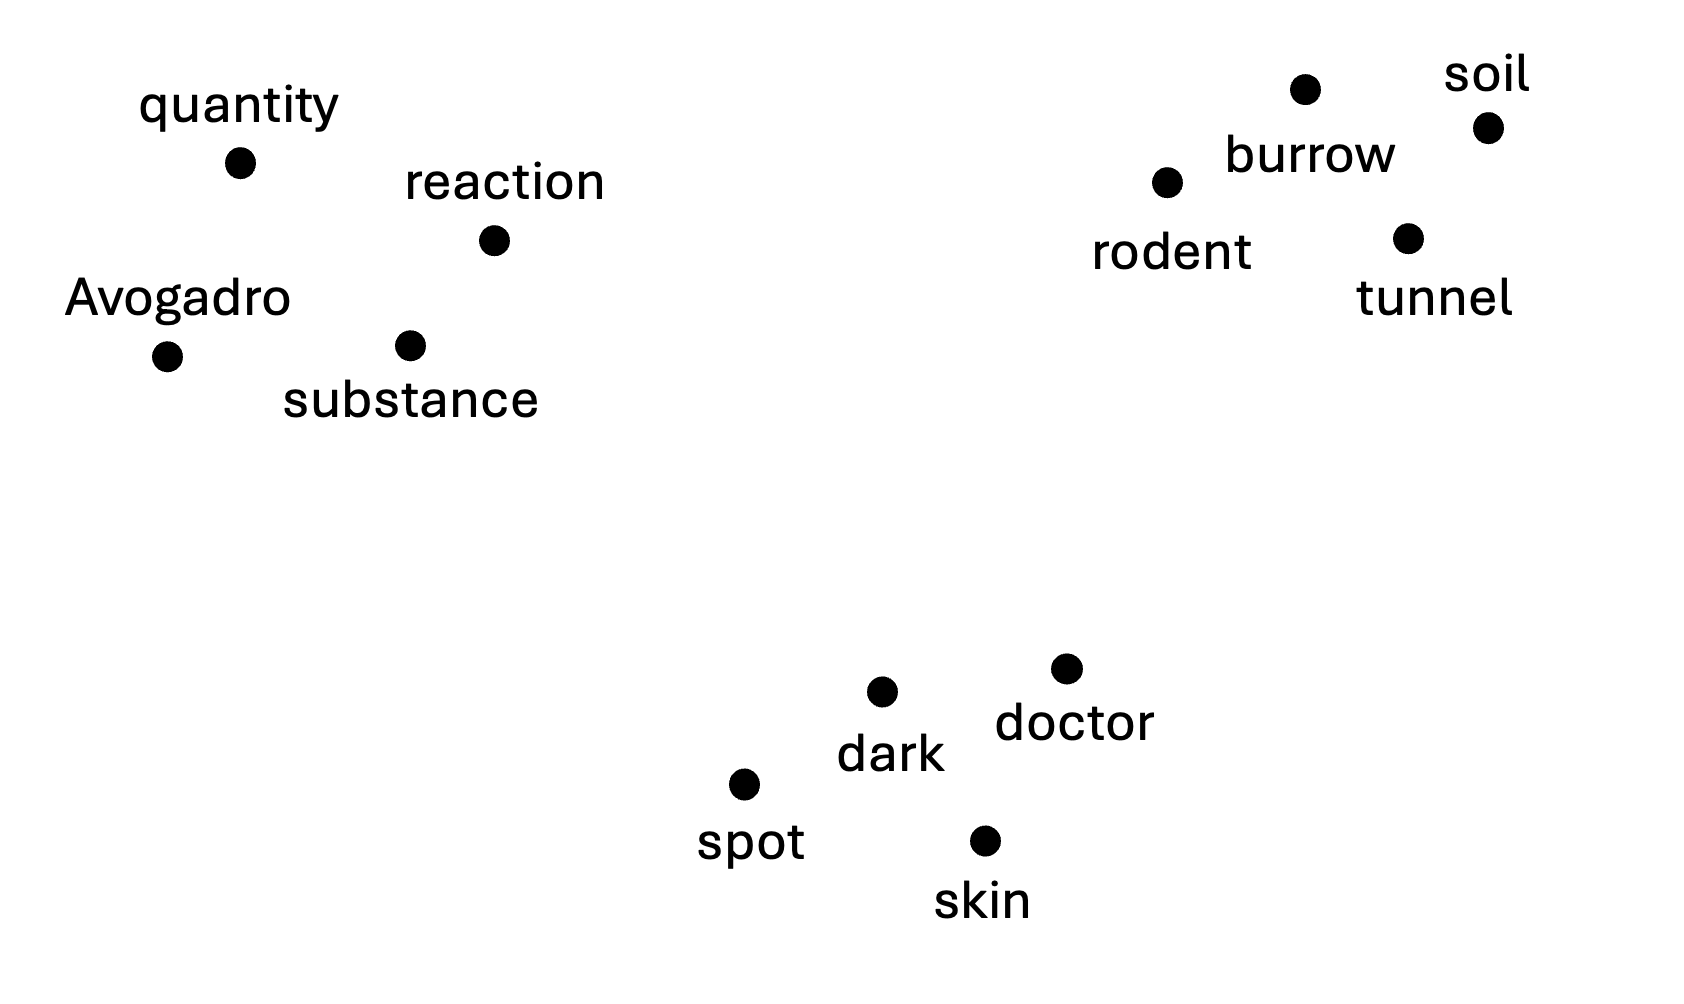
\includegraphics[width=\textwidth]{Figures/LLMs_work/embedding_contexts.png}
\end{figure}

\begin{solution}
the solution is not unique. One would argue that the most commonly used meaning of the word \textit{mole} is the skin spot or the animal. Thus, the student should place the word on the bottom cluster (skin spot) or the right cluster (animal). The exact position does not matter, it is enough if it is within that cluster.
\end{solution}

Now, given the following sentence (which we call \textbf{context}):

\vspace{0.5cm}
\textit{``One mole of any substance contains $6.022\cdot 10^{23}$ particles, which is known as Avogadro’s number"}
\vspace{0.5cm}

\textcolor{maincolor}{\textbf{\faPen\ b) Change the position of the word mole from the one you picked above to the one that better fits the given context.}} Keep the old position marked.

\begin{solution}
    the new position should be on the left cluster (it does not matter where exactly), the one related to Avogadro's number.
\end{solution}

\vspace{0.3cm}
\textcolor{maincolor}{\textbf{\faPen\ c) Draw an arrow between the old and the new positions of mole.}} This arrow is the transformation of the initial embedding of the word mole when taking a context into account. 


\exercisetitle{ Be an LLM}

Now, using the idea of embedding from the previous exercises, you are going to go through the same process as an LLM to predict the next word in an incomplete sentence.

\begin{importantbox}
    Your goal as an LLM: predict the next word in an incomplete sentence.
\end{importantbox}

\vspace{0.5cm}
\textbf{\large STEPS:}

\vspace{0.5cm}
\textbf{\large 1. Embedding: }
\vspace{0.5cm}

\textcolor{maincolor}{\textbf{\faPen\ a) Place the following words in the grid below, grouped by meaning, as you did above.}}

Words: \textit{lion, traffic light, street, tiger, zebra, building, giraffe, cross, city, leopard, crocodile}

\begin{solution}
    there should be two separated clusters, one with the words (lion, tiger, zebra, giraffe, leopard, crocodile) and another one with the words (traffic light, street, building, cross, city). Of course, it can happen that some student realizes that zebra can be in both, since ``zebra crossing" is also an element of the city. This is ok, they can put the word in both clusters.
\end{solution}

\begin{figure}[H]
    \centering
			
\includegraphics[width=\textwidth]{Figures/LLMs_work/grid_gpt_generated.png}
\end{figure}

\question{Did you find it easy to put all those words in this 2D grid? What would happen if you had to create 4 groups of words instead? How do you think you could place all the words in the dictionary in this 2D grid?}

In general, if you had to place all the words in the dictionary, it is impossible to do it in 2D grids, since you will eventually put together words that have nothing to do with each other in meaning. This is the reason why you need more dimensions, not just two! \textbf{Current LLMs need more than 10000 dimensions!}

\begin{importantbox}
    Up to now, the LLM (that is you now) has just embedded some words into a grid, which is called creating a ``vector representation".
\end{importantbox}

\vspace{0.5cm}
\textbf{\large 2. Attention mechanism: }
\vspace{0.5cm}

\textcolor{maincolor}{\textbf{\faPen\ b) Given the following sentences (\textit{contexts}), mark the words that make the word ``zebra" have the meaning it has in the sentence.}}

\begin{enumerate}
    \item I went to a zoo last week and saw many animals, but my favourite one was the zebra.
    \item I crossed the street at the zebra...
\end{enumerate}

\begin{solution}
    again here, the students can mark different words, since all of them are important, and this is just based on their intuition. However, the words that should be marked as ``the most important" (they are the ones that change the context and meaning for the word zebra in the sentence) are given in brackets [...] below:

\begin{enumerate}
    \item I went to a [zoo] last week and saw many [animals], but my favourite one was the zebra.
    \item I [crossed] the [street] at the zebra...
\end{enumerate}
\end{solution}


\begin{importantbox}
    What you are doing here is marking (or ``paying more attention to") the words in the sentences that modify the meaning of zebra in that context.
\end{importantbox}

Now, we are going to pick sentence number 2:

\vspace{0.5cm}
\textbf{\textit{``I crossed the street at the \colorbox{orange!30}{zebra}...."}}
\vspace{0.5cm}

This is the sentence that is incomplete. \textbf{Your goal as an LLM is to predict the word that follows ``zebra" in that sentence.}

\vspace{0.3cm}
\textcolor{maincolor}{\textbf{\faPen\ c) First go to the grid above in assignment 3a) and move the position of the zebra embedding to fit better the context of the sentence ``I crossed the street through the zebra....".}} Hint: Use the words you marked in part (b) (the ones you have to pay attention to) to get an idea of the words that should be closer to the new position (embedding) of zebra.

\begin{solution}
    considering that with high probability, the students have initially placed zebra together with the other animals, they now have to move its position to the cluster for words related to the city (analogously to what we did in Assignment 2.b)
\end{solution}

\begin{importantbox}
    You have now taken into account the context (the words you paid attention to) to change the representation of the word ``zebra".
\end{importantbox}

\vspace{0.5cm}
\textbf{\large 3. Prediction: }
\vspace{0.5cm}

Once you have taken into account the context of the sentence, it is time to predict the next word.

\question{Which word do you think follows in the sentence ``I crossed the street at the zebra..."?}

\begin{solution}
    The most likely word that comes after zebra is ``crossing".

    Complete sentence: I crossed the street at the zebra crossing.
\end{solution}

After having taken into account the context, and moved the representation of ``zebra" accordingly, the actual LLM uses a trained neural network to make the prediction. This neural network is shown a lot of examples of many different texts from the internet, from which it \textit{learns} to associate words to their most likely prediction. 

In the grid, the neural network ``moves'' the point representing ``zebra'' around until its final position. This final position is ``closer" to some words than others. Then, the LLM assigns higher probability to those words that are closer and lower probability to the words that are farther. Finally, it chooses the predicted word based on those probabilities.

All of that, you do intuitively, since you already have a lot of knowledge that you acquired through experience, and you don't even need to assign probabilities for each word, you just know.

\begin{importantbox}
    You can predict the next word `intuitively' because you have gained a lot of experience with language. The actual LLM trains a neural network with examples from texts in the internet to make the final prediction.
\end{importantbox}


\vspace{0.3cm}
\textcolor{maincolor}{\textbf{\faPen\ d) Create a prompt (anything that comes to your mind) and paste it in two different chats of an LLM.}} Does it give you the same answer in both?

\begin{importantbox}
    For the same input text, the final prediction is not always the same. The reason for this is that the LLM assigns probabilities for each possible word that comes next and then picks the word based on them. The choice is thus probabilistic.
\end{importantbox}

\exercisetitle{ LLM's learning}

One of the main differences between LLMs and other computer programs is that LLMs \textit{learn}. In other computer programs, the programmer needs to tell the machine what to do in \textit{all} the possible cases that the machine may encounter. For language, this would imply having to tell the computer what to reply to each possible prompt that the user writes.

This is not how LLMs operate. They learn from examples and then reply autonomously to each possible prompt that the user writes, without the programmer needing to do anything.

\question{Which of the steps that you have done in Assignment 3 do you think the LLM has to learn? Think of all the steps in which you used your intuition.}


The process above that you have done intuitively, the LLM needs to learn how to do it. It needs to learn all the steps:

\begin{itemize}
\item How to best embed the words.

\item How to pay attention to the important words in a sentence, those that may change its meaning (context).

\item How to change the embedding of the word depending on the context.

\item How to then predict which is the next word, for which it learns a transformation of the vector (it learns to change the position again, adding previous knowledge that it may already have).

\end{itemize}

After all this, it needs to go back from those vector embeddings into the tokens and assign a probability to each token. Finally, based on those probabilities, it selects one token and then transforms it into a word to complete the sentence.

\vspace{0.5cm}
\textbf{\large How does it learn all those things?}

By seeing tons and tons of examples of sentences from text in the internet. The analogy to how it does it is as follows: the LLM takes a sentence from the internet, ``covers" the part that it wants to predict, then makes the prediction, and finally ``uncovers" the sentence to check how good its prediction was. Then, it readjusts its internal mechanisms based on that feedback, and it gets better and better in its predictions the more data it gets. This way, it learns word patterns (which words typically go together), and how to move in the embedding grid based on ``concepts" (like the concept of ``wild animal", as we did when we linked with arrows the ``wild" versions of certain animals).

The actual way is more technical and less visual than what we have presented here, but we focused on understanding the main ideas behind it.

\end{document}